%\section{Game Control and Decision-making}
%
%	\subsection{Game Controller}
%	\paragraph{}
%	To control the operation during the game, all robots continuously receive the message from the referee’s game controller. When the received message indicates the change of	the game state, the current operation is terminated. Then the robot loads the new operation which associated with that state.
%	
%	\subsection{Decision Making System}
%	\paragraph{}
%	The decision making system of all striker robots can be described by the finite state machine illustrated in figure below. The conditions for state changes of each state are determined based on the observation data from the vision system and internal sensor reading of the robot. In addition, the robot shares this information among the teammates
%	by broadcasting mechanism via WLAN network. Therefore, the robot can cooperate to score the game as a team. The goalie decision can be described in a simpler state machine. The goalie is looking for the ball, if the ball heads toward the goalie on either direction (left/right). The goalie will fall in that direction in order to block the ball.
%	\begin{figure}[H]
%		\centering
%		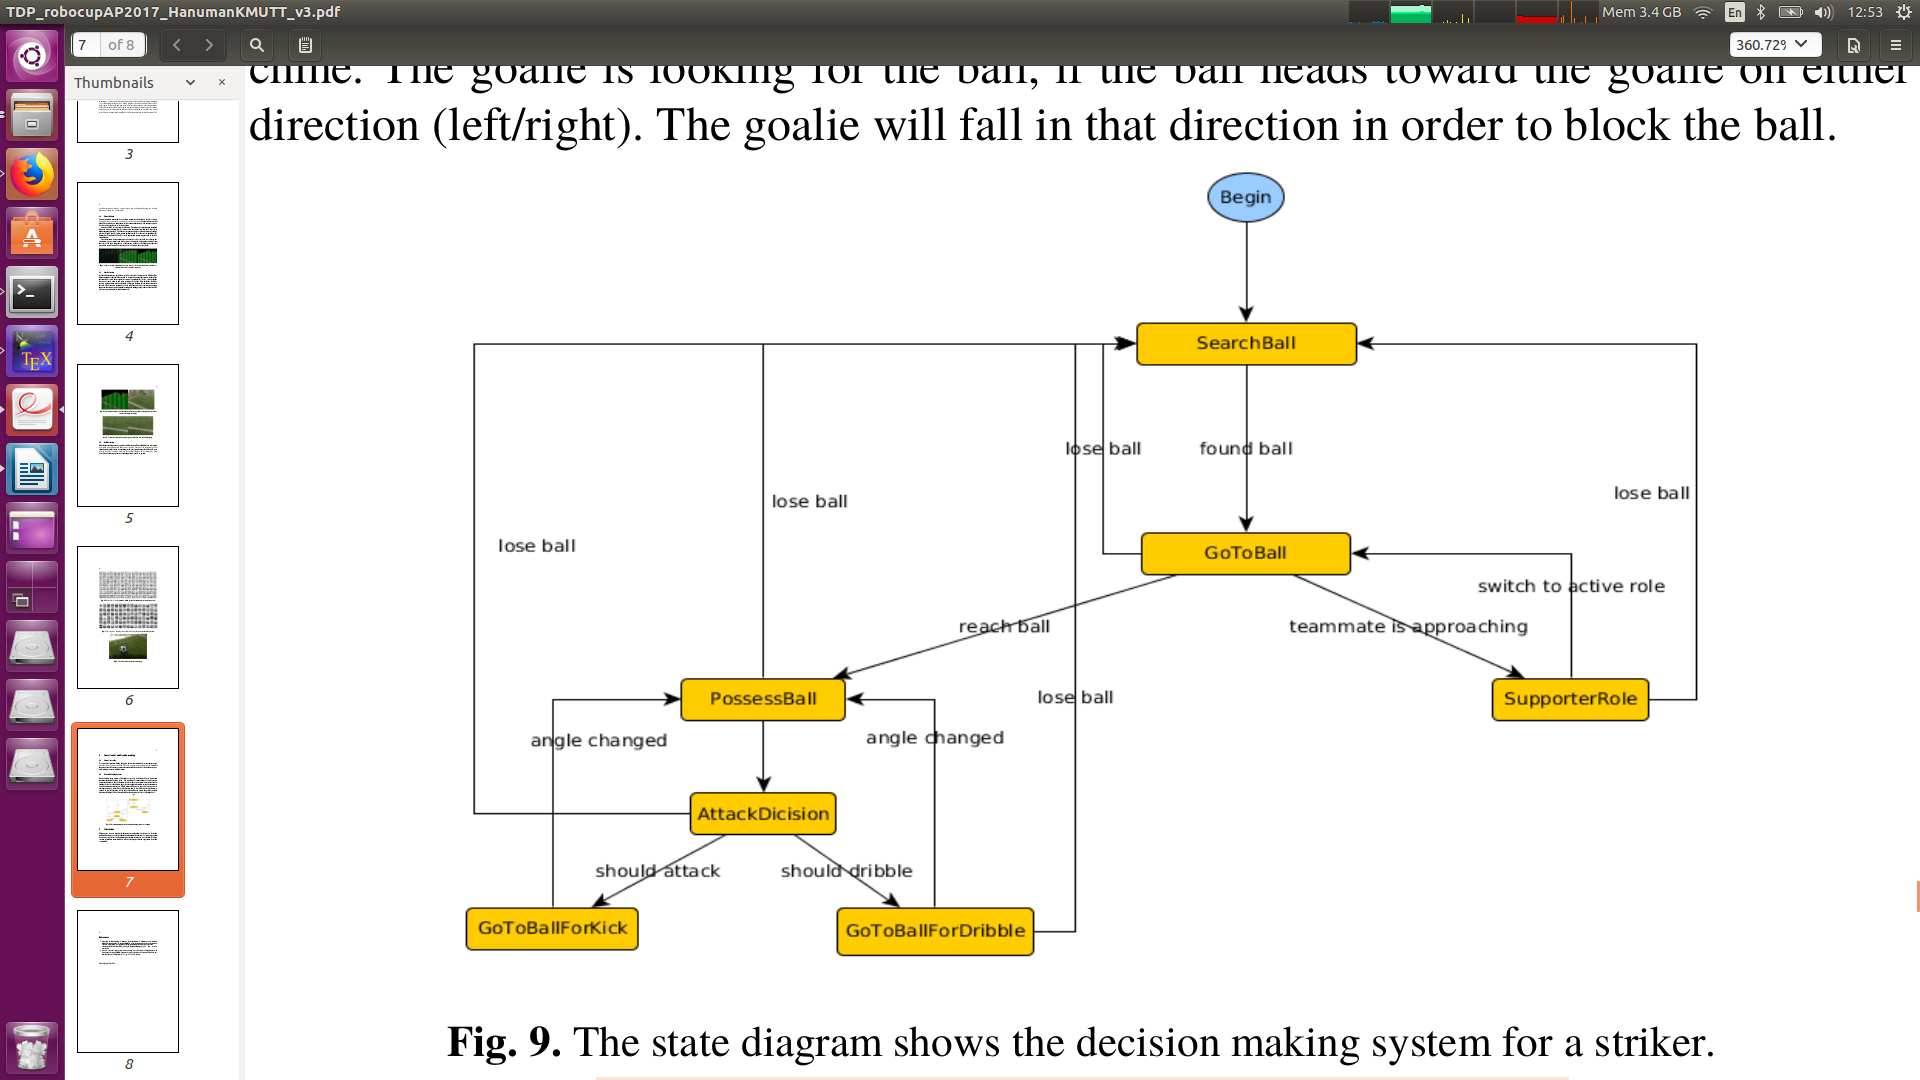
\includegraphics[width=\textwidth,trim={15cm 3cm 5cm 5.2cm},clip]{image/stateMachine.png}
%		\caption{The state diagram shows the decision making system for a striker.}
%		\label{fig:stateMachine}
%	\end{figure}